\documentclass[10pt, aspectratio=169]{beamer}
% Shared setup for every day of the course.
\usetheme[progressbar=frametitle, numbering=fraction, block=fill]{metropolis}
\usepackage[T1]{fontenc}
\usepackage[utf8]{inputenc}
\usepackage{lmodern}
\usepackage{amsmath, amssymb, bm, booktabs, graphicx, xcolor}
\usepackage{tikz}
\usetikzlibrary{arrows.meta, positioning, calc, shapes.geometric}

\graphicspath{{figures/}}

% --- colours -------------------------------------------------------------------------------------
\definecolor{accent}{HTML}{C0392B}
\definecolor{cool}{HTML}{2E6DB4}
\definecolor{muted}{HTML}{7A7A7A}
\definecolor{good}{HTML}{2E8B57}
\setbeamercolor{alerted text}{fg=accent}
\setbeamercolor{example text}{fg=cool}

% --- notation (follows the thesis' notation chapter) ---------------------------------------------
\newcommand{\given}{\,|\,}
\newcommand{\E}{\mathbb{E}}
\newcommand{\KL}[2]{D_{\mathrm{KL}}\!\left[#1\,\middle\|\,#2\right]}
\newcommand{\N}{\mathcal{N}}
\newcommand{\Hess}{\mathcal{H}}
\newcommand{\nats}{\,\text{nats}}
\DeclareMathOperator*{\argmin}{arg\,min}

% --- course devices ------------------------------------------------------------------------------
% \src{...}: where a claim or number comes from (thesis file and line, or a post-thesis note).
\newcommand{\src}[1]{\par\vfill\hfill{\scriptsize\color{muted}source: #1}}
% \wip: marks a post-thesis result.
\newcommand{\wip}{{\scriptsize\color{white}\colorbox{accent}{\,work in progress\,}}}
% \lesson{...}: the one sentence a frame exists to say.
\newcommand{\lesson}[1]{\begin{alertblock}{}\centering #1\end{alertblock}}
% a measurement story
\newenvironment{measured}[1]{\begin{exampleblock}{Measured: #1}}{\end{exampleblock}}

\author{Course built on the doctoral thesis of No\'e Zapata}
\institute{Montevideo, 30 November -- 4 December 2026}

% \cyclemap{n}: the course's five-stage cycle, stage n highlighted (1 room ... 5 memory).
\newcommand{\cyclemap}[1]{%
  \begin{tikzpicture}[
      st/.style={draw=muted, thick, rounded corners=3pt, fill=white, align=center,
                 minimum width=2.5cm, minimum height=0.8cm, font=\scriptsize, text=muted},
      on/.style={draw=accent, very thick, fill=accent!10, text=black, font=\scriptsize\bfseries},
      arr/.style={-{Stealth[length=2mm]}, thick, color=muted},
      s1/.style={}, s2/.style={}, s3/.style={}, s4/.style={}, s5/.style={}, s#1/.style={on}]
    \node[st, s1] (c1) at (90:1.9)   {estimate the room};
    \node[st, s2] (c2) at (18:2.6)   {localise; learn\\the body};
    \node[st, s3] (c3) at (-54:2.2)  {concepts fill\\the room};
    \node[st, s4] (c4) at (-126:2.2) {cross the door};
    \node[st, s5] (c5) at (162:2.6)  {new room;\\memory};
    \draw[arr] (c1) to[bend left=15] (c2); \draw[arr] (c2) to[bend left=15] (c3);
    \draw[arr] (c3) to[bend left=15] (c4); \draw[arr] (c4) to[bend left=15] (c5);
    \draw[arr] (c5) to[bend left=15] (c1);
  \end{tikzpicture}}


\title{A robot that acts to know}
\subtitle{Day 4 --- Action}
\date{Thursday 3 December}

\tikzset{box4/.style={draw, rounded corners=3pt, thick, align=center, font=\footnotesize, minimum height=0.8cm},
         arr4/.style={-{Stealth[length=2.5mm]}, thick},
         lab4/.style={font=\scriptsize}}

\begin{document}

\maketitle

\begin{frame}{Today: from a belief to a motion, and back}
  \centering
  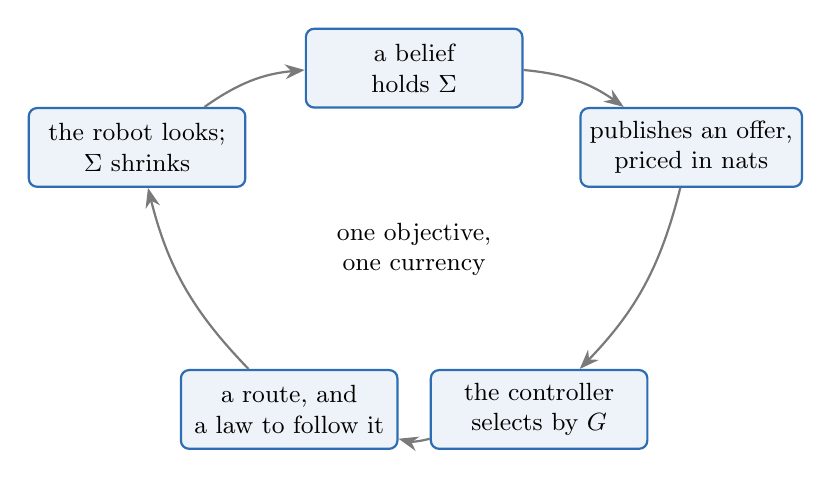
\begin{tikzpicture}[stage/.style={box4, draw=cool, fill=cool!8, minimum width=2.75cm, minimum height=1cm, font=\small}]
    \node[stage] (b) at (90:2.15) {a belief\\holds $\Sigma$};
    \node[stage] (o) at (18:3.7) {publishes an offer,\\priced in nats};
    \node[stage] (s) at (-54:2.7) {the controller\\selects by $G$};
    \node[stage] (r) at (-126:2.7) {a route, and\\a law to follow it};
    \node[stage] (l) at (162:3.7) {the robot looks;\\$\Sigma$ shrinks};
    \draw[arr4, color=muted] (b) to[bend left=15] (o);
    \draw[arr4, color=muted] (o) to[bend left=15] (s);
    \draw[arr4, color=muted] (s) to[bend left=15] (r);
    \draw[arr4, color=muted] (r) to[bend left=15] (l);
    \draw[arr4, color=muted] (l) to[bend left=15] (b);
    \node[align=center, font=\small] at (0,-0.15) {one objective,\\one currency};
  \end{tikzpicture}

  \small And at the end the robot turns the same objective on its own body.
\end{frame}

% Day 4: why action needs a second functional. \input from day4.tex.
% Frames moved from Day 1 on 2026-10-17. Figures d1_candidates.pdf / d1_diminishing.pdf are produced
% by figures/make_day1.py; d4_* by figures/make_day4.py.

% =================================================================================================
\section{Why action needs a second functional}
% =================================================================================================

\begin{frame}{Monday's frame, now done properly}
  \begin{columns}[c]
    \begin{column}{0.5\textwidth}
      \centering
      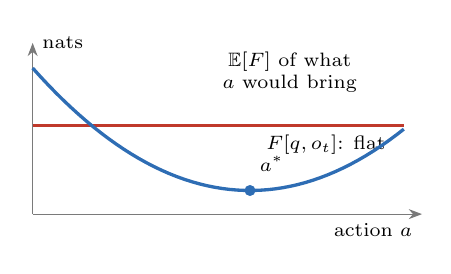
\begin{tikzpicture}[x=2.3cm, y=1.5cm, lab/.style={font=\scriptsize}]
        \draw[-{Stealth}, muted] (0,0) -- (2.15,0) node[below left, lab, text=black] {action $a$};
        \draw[-{Stealth}, muted] (0,0) -- (0,1.45) node[right, lab, text=black] {nats};
        \draw[accent, very thick] (0,0.75) -- (2.05,0.75);
        \node[lab, below] at (1.62,0.75) {$F[q,o_t]$: flat};
        \visible<2->{
        \draw[cool, very thick, domain=0:2.05, samples=50] plot (\x, {0.2 + 0.72*(\x-1.2)*(\x-1.2)});
        \fill[cool] (1.2,0.2) circle (2pt);
        \node[lab, above right] at (1.2,0.28) {$a^\ast$};
        \node[lab, align=center] at (1.42,1.2) {$\E[F]$ of what\\$a$ would bring};}
      \end{tikzpicture}
    \end{column}
    \begin{column}{0.46\textwidth}
      \textbf{Perception.} $o_t$ is fixed, so only $q$ can move.

      \vspace{0.6em}
      \textbf{Action.} At decision time $o_t$ is a number in a buffer:
      \[ \frac{\partial F[q,o_t]}{\partial a} = 0 . \]
      \pause
      What action \emph{can} change is the free energy of data not yet received:
      \[ a^\ast = \argmin_a \E_{q(o_{t+1},s_{t+1}\given a)}\big[F[q,o_{t+1}]\big] \]
    \end{column}
  \end{columns}
  \src{active\_inference.tex l.335--369}
\end{frame}

\begin{frame}{Expected free energy}
  For a policy $\pi$, with predicted states and observations $\tilde s,\tilde o$, and goals entering
  as a \textbf{prior over preferred outcomes} $p(\tilde o)$:
  \[ G(\pi) = \E_{q(\tilde s,\tilde o\given\pi)}\big[\ln q(\tilde s\given\pi) - \ln p(\tilde o,\tilde s)\big] \]
  Add and subtract $\ln q(\tilde s\given\tilde o,\pi)$, and split the joint. Exactly:
  \[
    G(\pi) = \E\Big[
      \underbrace{\ln q(\tilde s\given\pi) - \ln q(\tilde s\given\tilde o,\pi)}_{\text{epistemic}}
      \;\underbrace{-\ln p(\tilde o)}_{\text{pragmatic}}
      + \underbrace{\ln q(\tilde s\given\tilde o,\pi)-\ln p(\tilde s\given\tilde o)}_{\to 0 \text{ if inference stays good}}
    \Big]
  \]
  \lesson{No reward channel, no separate exploration bonus: both come out of the same line.}
  \src{active\_inference.tex l.371--412}
\end{frame}

\begin{frame}{Two terms, one currency}
  \centering
  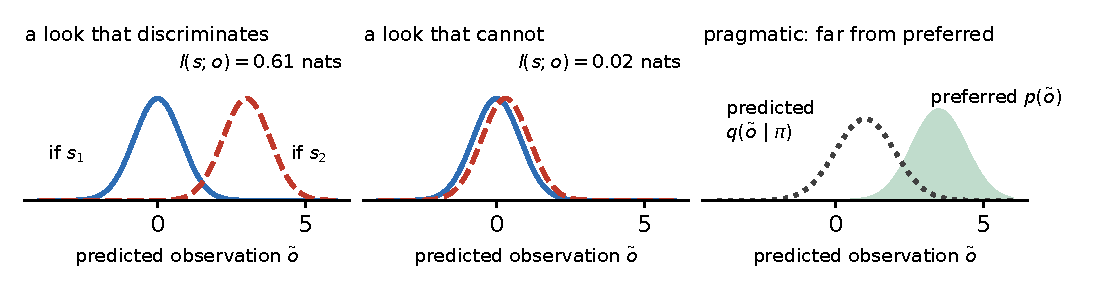
\includegraphics[width=0.97\textwidth]{d4_terms.pdf}

  \vspace{0.3em}
  \begin{columns}[T]
    \begin{column}{0.62\textwidth}
      \small
      \textbf{Epistemic} $=-I(\tilde s;\tilde o\given\pi)$: largest when what you would see depends on
      what is true.
    \end{column}
    \begin{column}{0.34\textwidth}
      \small
      \textbf{Pragmatic} $=-\E\ln p(\tilde o)$: what a cost function would have held.
    \end{column}
  \end{columns}

  \vspace{0.5em}
  \lesson{Both are in nats, derived together. The balance moves as the beliefs sharpen.}
  \src{active\_inference.tex l.414--427; curves: figures/make\_day4.py, block 1}
\end{frame}

\begin{frame}{For Gaussian beliefs, three names for one number}
  \begin{columns}[c]
    \begin{column}{0.36\textwidth}
      \centering
      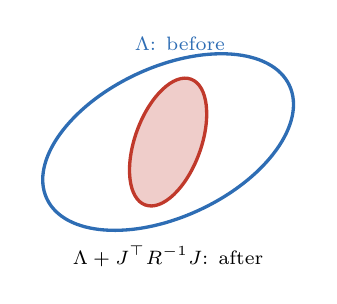
\begin{tikzpicture}
        \draw[cool, very thick, rotate=25] (0,0) ellipse (1.7cm and 0.95cm);
        \draw[accent, very thick, rotate=70, fill=accent!25] (0,0) ellipse (0.85cm and 0.42cm);
        \node[font=\scriptsize, text=cool] at (0.15,1.25) {$\Lambda$: before};
        \node[font=\scriptsize] at (0,-1.45) {$\Lambda + J^\top R^{-1}J$: after};
      \end{tikzpicture}\\[0.3em]
      {\small $\Delta H$ is the log of the area ratio.}
    \end{column}
    \begin{column}{0.6\textwidth}
      \[
        \underbrace{H[q]-\E H[q\given o]}_{\text{expected entropy drop}}
        = \underbrace{I(s;o)}_{\text{mutual information}}
      \]
      \[
        = \underbrace{\tfrac12\ln\frac{|\Lambda + J^\top R^{-1}J|}{|\Lambda|}}_{\text{D-optimal design}}
      \]
      \small
      The epistemic term, the information gain of active sensing and the criterion of optimal
      experiment design are \alert{one quantity}. It depends on \emph{where} you look, not on
      \emph{what} you will see, so it can be computed before moving.
    \end{column}
  \end{columns}
  \src{appendix\_math.tex l.742--779, l.1236--1287}
\end{frame}

\begin{frame}{Where to look next}
  \begin{columns}[c]
    \begin{column}{0.58\textwidth}
      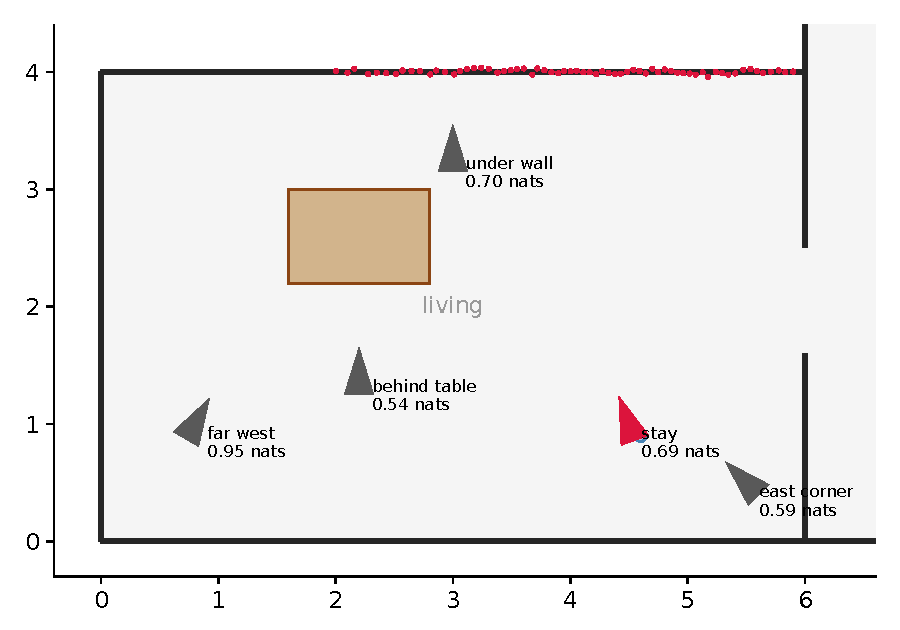
\includegraphics[width=\textwidth]{d1_candidates.pdf}
    \end{column}
    \begin{column}{0.4\textwidth}
      \small
      Monday's wall: the robot (red) has seen its east part. Five candidate viewpoints.
      \begin{itemize}
        \item ``far west'' sees few points and gains the most: it adds lever arm where the
              information is weak;
        \item ``stay'' gains exactly $\ln 2$. Why?
      \end{itemize}
    \end{column}
  \end{columns}
  \src{lab 4, exercise 1}
\end{frame}

\begin{frame}{Diminishing returns, and a warning}
  \begin{columns}[c]
    \begin{column}{0.45\textwidth}
      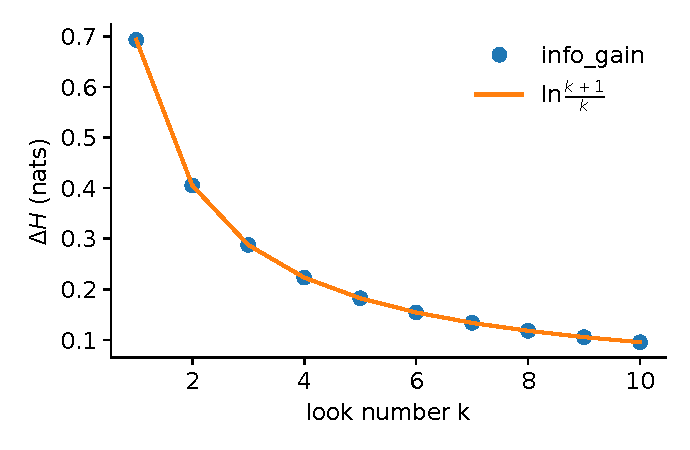
\includegraphics[width=\textwidth]{d1_diminishing.pdf}
    \end{column}
    \begin{column}{0.53\textwidth}
      \small
      The $k$-th identical look gives $|(k{+}1)\Lambda_1| / |k\Lambda_1|=((k{+}1)/k)^2$ for two
      parameters, so
      \[ \Delta H_k = \ln\frac{k+1}{k}. \]
      \pause
      \alert{But this assumes each look's errors are independent.} Repeated looks share the pose
      and the calibration, and those do not average away.\\[0.4em]
      Day 3's common-mode ceiling already put a number on how little a repeat look is worth.
    \end{column}
  \end{columns}
  \src{lab 4, exercise 2}
\end{frame}


% =================================================================================================
\section{Affordances: published, priced offers}
% =================================================================================================

\begin{frame}{Each term of $G$ belongs to the process that can compute it}
  \centering
  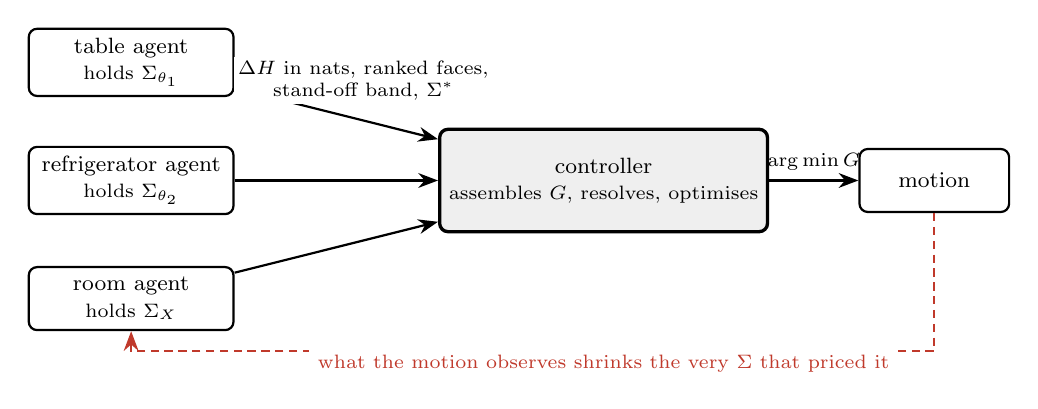
\begin{tikzpicture}[p/.style={box4, minimum width=2.6cm}]
    \node[p] (t) at (0,1.5) {table agent\\{\scriptsize holds $\Sigma_{\theta_1}$}};
    \node[p] (f) at (0,0) {refrigerator agent\\{\scriptsize holds $\Sigma_{\theta_2}$}};
    \node[p] (r) at (0,-1.5) {room agent\\{\scriptsize holds $\Sigma_X$}};
    \node[box4, very thick, fill=muted!12, minimum width=3.6cm, minimum height=1.3cm] (c) at (6.0,0) {controller\\{\scriptsize assembles $G$, resolves, optimises}};
    \node[box4, minimum width=1.9cm] (m) at (10.2,0) {motion};
    \foreach \a in {t,f,r} \draw[arr4] (\a) -- (c);
    \draw[arr4] (c) -- node[above, lab4] {$\argmin G$} (m);
    \node[lab4, align=center, fill=white, inner sep=1.5pt] at (2.95,1.27) {$\Delta H$ in nats, ranked faces,\\stand-off band, $\Sigma^\ast$};
    \draw[arr4, densely dashed, accent] (m.south) -- ++(0,-1.75) -| (r.south);
    \node[lab4, text=accent, align=center, fill=white] at (6.0,-2.32) {what the motion observes shrinks the very $\Sigma$ that priced it};
  \end{tikzpicture}

  \vspace{0.5em}
  \small An offer is a node in the graph. Add a class of object and you add terms to $G$;
  the controller does not change.
  \src{action.tex l.78--84, l.146--188, l.1478--1481}
\end{frame}

\begin{frame}{The split of knowledge}
  \begin{columns}[c]
    \begin{column}{0.44\textwidth}
      \centering
      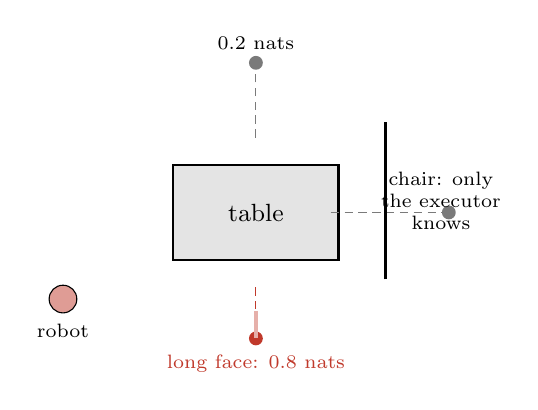
\begin{tikzpicture}
        \draw[thick, fill=muted!20] (-1.05,-0.6) rectangle (1.05,0.6);
        \node[font=\small] at (0,0) {table};
        \foreach \a/\r/\col in {-90/1.6/accent, 90/1.9/muted, 0/2.45/muted} {
          \draw[densely dashed, color=\col] (\a:0.95) -- (\a:\r);
          \fill[color=\col] (\a:\r) circle (2.5pt);
        }
        \node[lab4, text=accent] at (-90:1.92) {long face: 0.8 nats};
        \node[lab4] at (90:2.15) {0.2 nats};
        \draw[very thick, accent!40] (-90:1.25) -- (-90:1.6);
        \fill[accent!50, draw=black] (-2.45,-1.1) circle (5pt);
        \node[lab4] at (-2.45,-1.5) {robot};
        \draw[very thick] (1.65,-0.85) -- (1.65,1.15);
        \node[lab4, align=center] at (2.35,0.15) {chair: only\\the executor\\knows};
      \end{tikzpicture}
    \end{column}
    \begin{column}{0.53\textwidth}
      \renewcommand{\arraystretch}{1.5}
      \small
      \begin{tabular}{@{}p{2.1cm} p{4.5cm}@{}}
        \toprule
        \textbf{producer} & which view, \emph{relative to its object}; what it is worth; when it has learnt enough ($\Sigma^\ast$) \\
        \textbf{executor} & feasibility; the cost of getting there; how to move and stop \\
        \bottomrule
      \end{tabular}

      \vspace{0.8em}
      A producer cannot publish a world pose. A demand that may be impossible has no vocabulary for
      saying so; a constraint can be negotiated.
    \end{column}
  \end{columns}
  \src{action.tex l.42--45, l.109--122}
\end{frame}

\begin{frame}{The price of a view}
  \centering
  \[
    \E[\Delta H](\mathbf v) \;=\; P(\text{detect}\given\mathbf v)\;\sum_j\tfrac12\ln\!\Big(1+\frac{I_j(\mathbf v)}{Y_j}\Big)
  \]
  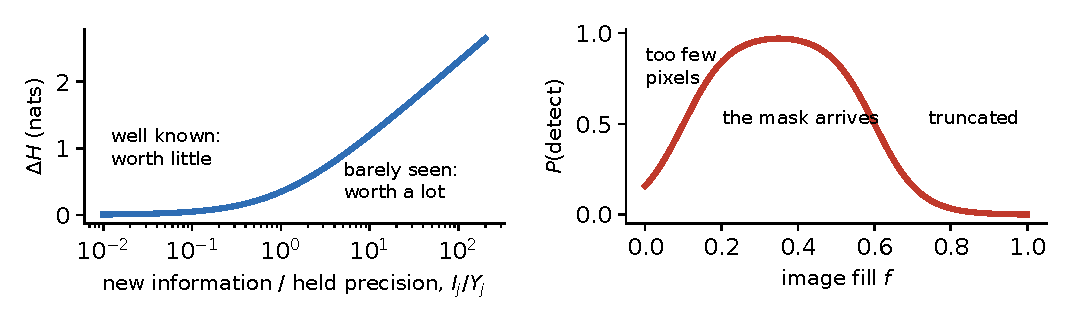
\includegraphics[width=0.74\textwidth]{d4_currency.pdf}

  \raggedright\small
  $f_{\min}{=}0.10$, $f_{\max}{=}0.60$, $w_f{=}0.06$ are a prior, not a measurement. And because the
  band is unimodal, a robot unsure of an object's size stands further back: no margin was set.
  \src{action.tex l.193--207, l.218--226, l.256--265}
\end{frame}

\begin{frame}{Selecting: one comparison, every cycle}
  \[
    a^\star = \argmin_a\big[\lambda\cdot\mathrm{dist}(a) - \Delta H(a) - \text{pragmatic}(a)\big],
    \qquad \lambda = 0.2\ \text{nats/m}
  \]
  \begin{columns}[c]
    \begin{column}{0.56\textwidth}
      \centering
      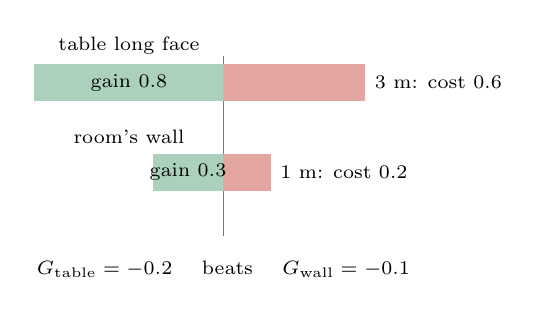
\begin{tikzpicture}[x=3.0cm, y=0.95cm, lab/.style={font=\scriptsize}]
        \draw[muted] (0,-0.3) -- (0,2.1);
        \foreach \y/\n/\g/\c in {1.5/table long face/0.8/0.6, 0.3/room's wall/0.3/0.2} {
          \fill[good!40] (0,\y) rectangle (-\g,\y+0.5);
          \fill[accent!45] (0,\y) rectangle (\c,\y+0.5);
          \node[lab, above] at (-0.4,\y+0.5) {\n};
          \node[lab] at (-\g/2,\y+0.25) {gain $\g$};
        }
        \node[lab, right] at (0.6,1.75) {3 m: cost 0.6};
        \node[lab, right] at (0.2,0.55) {1 m: cost 0.2};
        \node[lab, align=center] at (0,-0.75) {$G_{\text{table}} = -0.2$ \quad beats \quad $G_{\text{wall}} = -0.1$};
      \end{tikzpicture}
    \end{column}
    \begin{column}{0.4\textwidth}
      \small
      Illustrative gains.\\[0.3em]
      Already driving to the wall? The table must win by a \textbf{switching margin},
      $0.5$ nats: the price of work already invested.
      \begin{itemize}
        \item It is inside $G$, not a gate on it.
        \item The offer in hand is re-scored with the rest.
      \end{itemize}
    \end{column}
  \end{columns}
  \src{action.tex l.42--49, l.329--347}
\end{frame}

\begin{frame}{An offer loses value by succeeding}
  \centering
  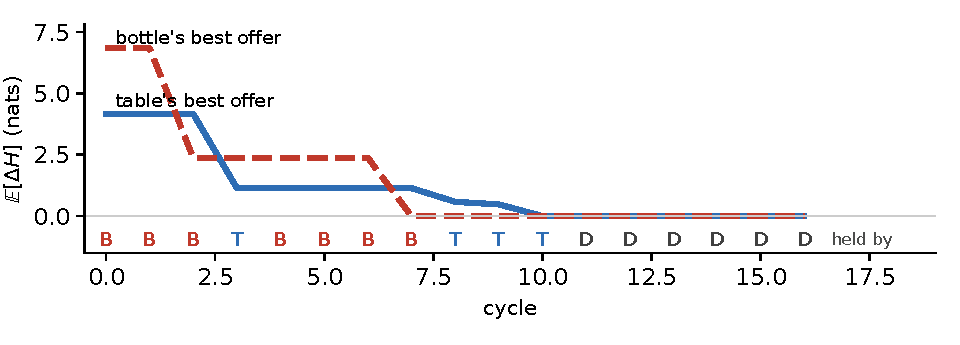
\includegraphics[width=0.66\textwidth]{d4_handoff.pdf}

  \raggedright\small
  The toy of today's lab: two producers and a door worth 1 nat of preference. Nobody wrote
  ``the table is done, go to the bottle''. Each look shrinks the covariance that priced the look,
  until another offer is better by more than the margin.
  \lesson{Interruption is a consequence of the values, not a rule in the executor.}
  \src{action.tex l.347--353; lab 4, exercise 7}
\end{frame}

\begin{frame}{The room: predict through everything you believe}
  \centering
  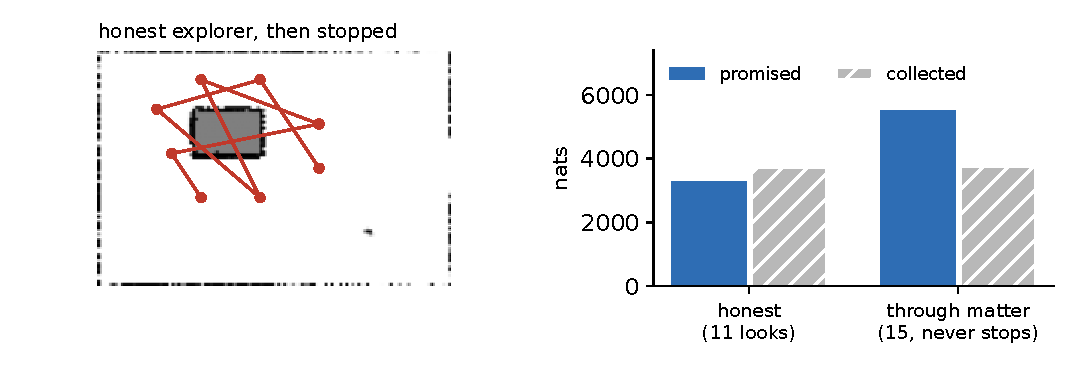
\includegraphics[width=0.84\textwidth]{d4_explorer.pdf}

  \raggedright\small
  An explorer that casts its predicted beams through what it already knows is solid promises
  cells nobody can reach, collects nothing for them, and offers them again at the next decision: the
  robot would shuttle between two standpoints.
  \alert{Predicted against realised gain is the most useful diagnostic an explorer has.}
  \src{layout\_acquisition.tex l.725--728; lab 4, exercises 8--10}
\end{frame}

\begin{frame}{What is not established}
  \begin{columns}[T]
    \begin{column}{0.5\textwidth}
      \begin{measured}{derived objective against a heuristic}
        \small
        The explorer written in nats, no free weights, against the hand-tuned scorer, over a
        population of simulated rooms: \textbf{indistinguishable in the mean}. It made a majority of
        rooms slightly worse and rescued a few outright failures.
      \end{measured}
      \small
      The explorer running now scores unseen floor per metre: a coverage rule.
    \end{column}
    \begin{column}{0.46\textwidth}
      \small
      \textbf{Still design, not mechanism:}
      \begin{itemize}
        \item the horizon is one affordance deep: the next look, not the best order;
        \item the pragmatic channel is thin;
        \item an offer completes on a detection, not on reaching $\Sigma^\ast$.
      \end{itemize}
      \alert{The case for the derived form rests on its having no free parameters, not on performance.}
    \end{column}
  \end{columns}
  \src{active\_inference.tex l.876--897; action.tex l.1420--1436}
\end{frame}

% =================================================================================================
\section{From a choice to a motion}
% =================================================================================================

\begin{frame}{Who answers for obstacles? The geometry}
  \centering
  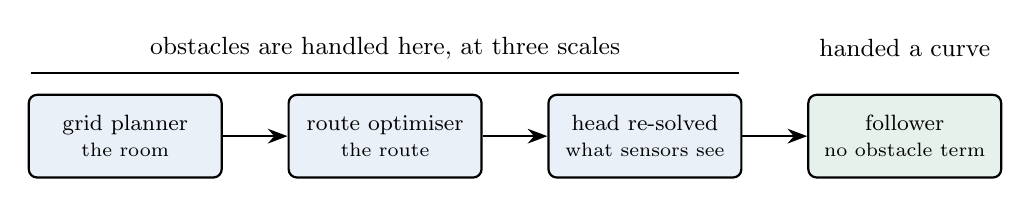
\begin{tikzpicture}[s/.style={box4, minimum width=2.45cm, minimum height=1.05cm}]
    \node[s, fill=cool!10] (a) at (0,0) {grid planner\\{\scriptsize the room}};
    \node[s, fill=cool!10] (b) at (3.3,0) {route optimiser\\{\scriptsize the route}};
    \node[s, fill=cool!10] (c) at (6.6,0) {head re-solved\\{\scriptsize what sensors see}};
    \node[s, fill=good!12] (d) at (9.9,0) {follower\\{\scriptsize no obstacle term}};
    \draw[arr4] (a) -- (b); \draw[arr4] (b) -- (c); \draw[arr4] (c) -- (d);
    \draw[thick] (-1.2,0.8) -- (7.8,0.8);
    \node[font=\small] at (3.3,1.12) {obstacles are handled here, at three scales};
    \node[font=\small, align=center] at (9.9,1.12) {handed a curve};
  \end{tikzpicture}

  \vspace{1em}
  \begin{columns}[T]
    \begin{column}{0.48\textwidth}
      \small
      The follower has no avoidance mode and no arbitration between avoiding and tracking.
      An arbitration problem has become a \textbf{coverage requirement}.
    \end{column}
    \begin{column}{0.48\textwidth}
      \small
      Others choose differently: timed elastic bands emit the commands themselves; predictive
      contouring keeps obstacles in the controller; regulated pure pursuit carries a collision check,
      the price of replanning at 1 Hz and tracking at 20.
    \end{column}
  \end{columns}
  \src{action.tex l.985--1008}
\end{frame}

\begin{frame}{Routes as optimisation}
  \[
    J[r] = w_c\,\underbrace{\big\langle u^2+4u^4\big\rangle}_{\text{clearance}}
    + w_\kappa\,\underbrace{\big\langle(\rho\kappa)^2\big\rangle}_{\text{bending}}
    + \lambda_a\underbrace{\textstyle\sum_k\mathrm{Huber}(\delta_k)}_{\text{authored waypoints}}
    + \lambda_j\,\underbrace{\big\langle(\mathrm{d}\kappa/\mathrm{d}s)^2\big\rangle}_{\text{turn-rate roughness}}
  \]
  \begin{columns}[c]
    \begin{column}{0.5\textwidth}
      \small
      \begin{itemize}
        \item The quartic: margin is surrendered only where it is plentiful.
        \item $\rho=v_{\max}^2/a^{\max}_{\mathrm{lat}}$: bending is priced by the speed it costs.
        \item Terms are \emph{not} normalised by their current size, so re-optimising an optimal
              route leaves it alone.
      \end{itemize}
    \end{column}
    \begin{column}{0.46\textwidth}
      \centering\small
      \begin{tabular}{@{}l r r@{}}
        \toprule
        fixed tour & before & after \\
        \midrule
        5th-pct.\ clearance (m) & 0.334 & 0.431 \\
        lap time (s)            & 131.3 & 116.8 \\
        waypoint fidelity (m)   & 0.115 & 0.173 \\
        \bottomrule
      \end{tabular}

      \vspace{0.3em}
      {\scriptsize The third row is the price; an earlier speed limit, before $\lambda_j$.}
    \end{column}
  \end{columns}
  \src{action.tex l.837--876, l.878--904}
\end{frame}

\begin{frame}{The error, in the curve's own coordinates}
  \begin{columns}[c]
    \begin{column}{0.5\textwidth}
      \centering
      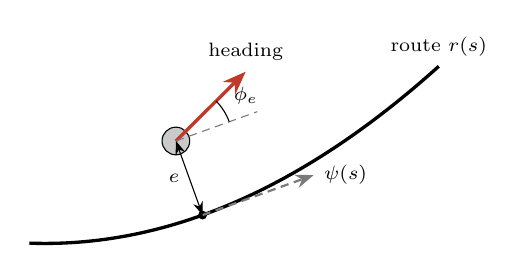
\begin{tikzpicture}[x=1cm, y=1cm]
        \draw[very thick] plot[domain=-0.2:5.0, samples=60] (\x, {0.09*\x*\x});
        \coordinate (F) at (2,0.36);
        \coordinate (R) at (1.661,1.301);
        \fill (F) circle (1.6pt);
        \draw[densely dashed, muted, thick, -{Stealth}] (F) -- ++(19.8:1.5) node[right, lab4, text=black] {$\psi(s)$};
        \fill[muted!40, draw=black] (R) circle (5pt);
        \draw[-{Stealth}, very thick, accent] (R) -- ++(44.8:1.25) node[above, lab4, text=black] {heading};
        \draw[densely dashed, muted] (R) -- ++(19.8:1.1);
        \draw ([shift=(19.8:0.72)]R) arc (19.8:44.8:0.72);
        \node[lab4] at (2.55,1.88) {$\phi_e$};
        \draw[{Stealth}-{Stealth}] (F) -- node[left, lab4] {$e$} (R);
        \node[lab4] at (5.0,2.5) {route $r(s)$};
      \end{tikzpicture}
    \end{column}
    \begin{column}{0.46\textwidth}
      \[
        \dot e \approx v\,\phi_e,
        \qquad
        \dot\phi_e = \omega - v\,\kappa(s)
      \]
      \small
      Heading error turns forward motion into sideways drift. Heading error grows by whatever turn
      rate exceeds what the curve demands.\\[0.5em]
      Which suggests the law:
      \[
        \omega = \underbrace{v\kappa(s)}_{\text{feedforward}}
        - v\Big(\frac{2}{L}\,\phi_e+\frac{1}{L^2}\,e\Big)
      \]
    \end{column}
  \end{columns}
  \src{action.tex l.1019--1027, l.1069--1077}
\end{frame}

\begin{frame}{A law you can write down}
  \begin{columns}[c]
    \begin{column}{0.48\textwidth}
      \begin{measured}{the earlier follower was a sampler}
        \small
        An offline replay found the lateral term contributing \textbf{91.6\%} of the sampler's cost:
        in effect a lateral regulator paying for $K$ rollouts. The tracker replaced it, and the
        sampler is gone from the build.
      \end{measured}
    \end{column}
    \begin{column}{0.48\textwidth}
      \small
      \textbf{The feedforward is exact.} The unicycle is differentially flat with respect to its
      position, so a $C^2$ curve and a speed profile fix $\omega=v\kappa$ in closed form.\\[0.6em]
      A sampler earns its cost with multimodal costs and obstacles inside the objective. Here the
      obstacles live in the route.
    \end{column}
  \end{columns}
  \vspace{0.6em}
  \lesson{When the dynamics are locally linear and one term dominates, write the law.}
  \src{action.tex l.1040--1046, l.1054--1062}
\end{frame}

\begin{frame}{Pole assignment: the gains are not tuned}
  \begin{columns}[c]
    \begin{column}{0.4\textwidth}
      \centering
      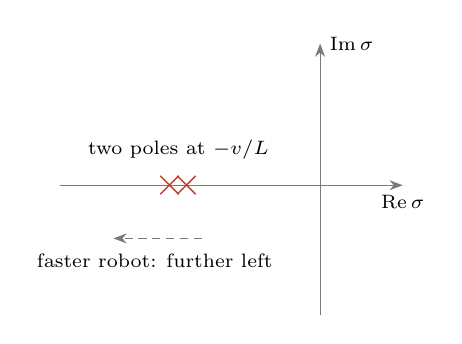
\begin{tikzpicture}[x=1.5cm, y=1.5cm]
        \draw[-{Stealth}, muted] (-2.2,0) -- (0.7,0) node[below, lab4, text=black] {$\mathrm{Re}\,\sigma$};
        \draw[-{Stealth}, muted] (0,-1.1) -- (0,1.2) node[right, lab4, text=black] {$\mathrm{Im}\,\sigma$};
        \node[accent, font=\Large] at (-1.2,0) {$\times\!\!\times$};
        \node[lab4, above] at (-1.2,0.14) {two poles at $-v/L$};
        \draw[densely dashed, muted, -{Stealth}] (-1.0,-0.45) -- (-1.75,-0.45);
        \node[lab4, below] at (-1.4,-0.5) {faster robot: further left};
      \end{tikzpicture}
    \end{column}
    \begin{column}{0.56\textwidth}
      Substituting the law into the error equations, at constant speed:
      \[
        \ddot e + \frac{2v}{L}\,\dot e + \frac{v^2}{L^2}\,e = 0
        \;\Longrightarrow\; (\sigma + v/L)^2 = 0
      \]
      \small
      Critically damped by construction, with one free parameter, because a double pole fixes both
      gains:
      \[ k_d = \frac{2}{L},\qquad k_p = \frac{v}{L^2}. \]
      $L = 0.50$ m. What was chosen is where the poles sit.
    \end{column}
  \end{columns}
  \src{action.tex l.1100--1109, l.1163--1181}
\end{frame}

\begin{frame}{The error decays over a distance, not a time}
  \centering
  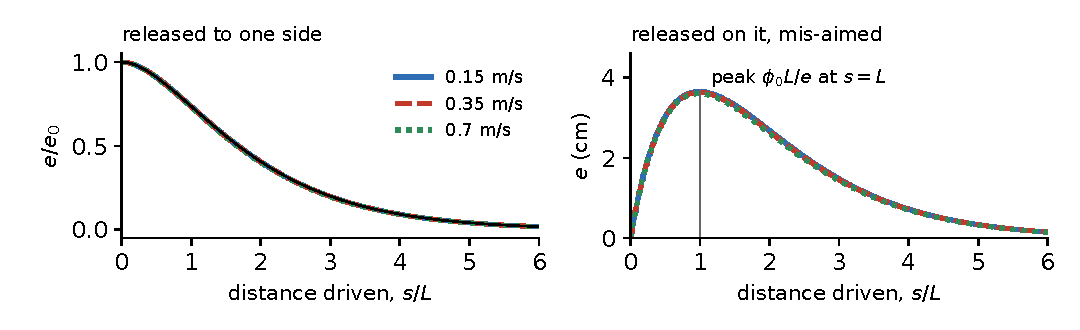
\includegraphics[width=0.76\textwidth]{d4_decay.pdf}

  \raggedright\small
  With $\mathrm{d}/\mathrm{d}t=v\,\mathrm{d}/\mathrm{d}s$ the speed cancels: $e(s)=(A+Bs)\,e^{-s/L}$.
  A robot crawling through a door and one crossing a room converge over the same metres, with no gain
  schedule. These are the toy's three speeds; thin black is the formula.
  \lesson{$L$ is not a gain. It is a length, read off the space the robot works in.}
  \src{action.tex l.1185--1198, l.1229--1236, l.1257--1260; lab 4, exercise 12}
\end{frame}

\begin{frame}{Why this follower needs no obstacle term}
  \centering
  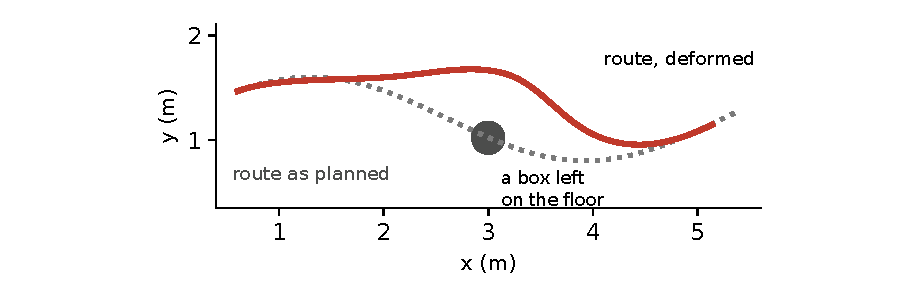
\includegraphics[width=0.8\textwidth]{d4_route.pdf}

  \raggedright\small
  Same follower, unchanged. Only the curve moved: clearance $-40$ cm straight through, $+23$ cm after
  deforming.\\[0.4em]
  \textbf{What it costs.} An obstacle outside the live field, or inside the short fixed prefix, is not
  avoided at all. \alert{No comparison with the window disabled has been run}: the
  window is justified by the division of labour, not by a measured benefit.
  \src{action.tex l.1002--1008; lab 4, exercise 14}
\end{frame}

\begin{frame}{Following and choosing are one objective, at two depths}
  \[
    \nabla_{u_t} G_T(\pi)
      = \underbrace{\nabla_{u_t} G_{t+1}(u_t)}_{\text{what the follower handles, in closed form}}
      + \underbrace{\sum_{\tau=t+2}^{t+T}\nabla_{u_t} G_\tau(\pi)}_{\text{what the selector adds, in affordances}}
  \]
  \begin{center}
  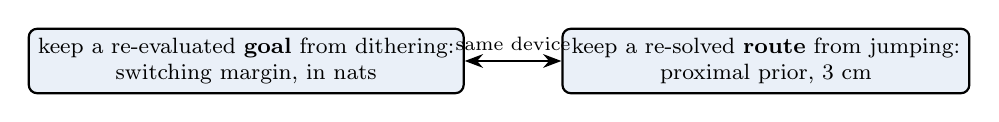
\begin{tikzpicture}[s/.style={box4, minimum width=4.5cm}]
    \node[s, fill=cool!10] (a) at (0,0) {keep a re-evaluated \textbf{goal} from dithering:\\switching margin, in nats};
    \node[s, fill=cool!10] (b) at (6.6,0) {keep a re-solved \textbf{route} from jumping:\\proximal prior, 3 cm};
    \draw[{Stealth}-{Stealth}, thick] (a) -- node[above, lab4] {same device} (b);
  \end{tikzpicture}
  \end{center}
  \small MPC, MPPI and planning as inference sit on this line, and differ in how many terms they keep
  and how they estimate them.
  \src{active\_inference.tex l.504--508, l.554--579; action.tex l.978, l.1396--1408}
\end{frame}

% =================================================================================================
\section{The same objective, turned on itself}
% =================================================================================================

\begin{frame}{Calibration is inference, not maintenance}
  \begin{columns}[c]
    \begin{column}{0.52\textwidth}
      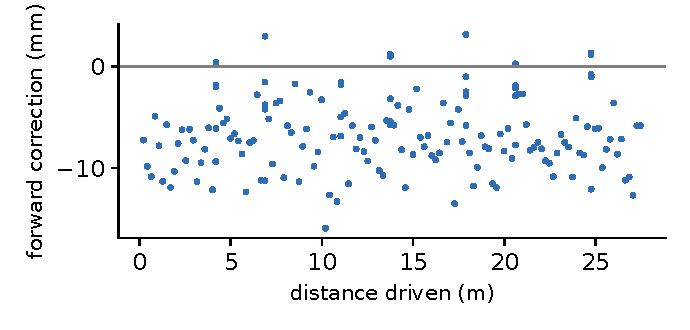
\includegraphics[width=\textwidth]{d4_sawtooth.pdf}
    \end{column}
    \begin{column}{0.44\textwidth}
      \small
      The toy's wheels over-report by 4\%. The room corrects each step, and every correction points the
      same way.\\[0.5em]
      A wider covariance would not help: it says how far the prediction may be wrong, not in
      \emph{which direction}.\\[0.5em]
      Put $(s_v,s_\omega,b)$ in the state: NEES $8.3\to1.6$.
    \end{column}
  \end{columns}
  \lesson{If the body is a factor of the posterior, estimating it is the same inference.}
  \src{active\_inference.tex l.797--800; self\_calibration.tex l.53; lab 4, exercises 15--17}
\end{frame}

\begin{frame}{What no data can determine}
  \begin{columns}[c]
    \begin{column}{0.47\textwidth}
      \centering
      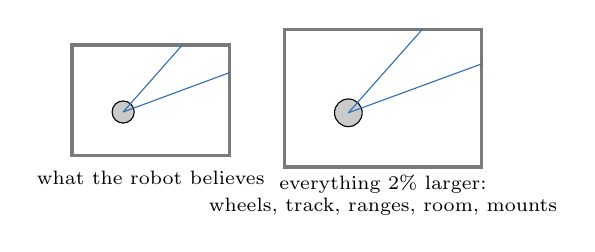
\begin{tikzpicture}
        \draw[very thick, muted] (0,0) rectangle (2.0,1.4);
        \fill[muted!40, draw=black] (0.65,0.55) circle (4pt);
        \draw[cool] (0.65,0.55) -- (2.0,1.05); \draw[cool] (0.65,0.55) -- (1.4,1.4);
        \node[lab4] at (1,-0.28) {what the robot believes};
        \draw[very thick, muted] (2.7,-0.15) rectangle (5.2,1.6);
        \fill[muted!40, draw=black] (3.51,0.54) circle (5pt);
        \draw[cool] (3.51,0.54) -- (5.2,1.16); \draw[cool] (3.51,0.54) -- (4.45,1.6);
        \node[lab4, align=center] at (3.95,-0.5) {everything 2\% larger:\\wheels, track, ranges, room, mounts};
      \end{tikzpicture}

      \vspace{0.5em}
      {\small No reading changes.}
    \end{column}
    \begin{column}{0.5\textwidth}
      A transformation that changes no factor of the model is a \textbf{gauge}. The data cannot fix
      it; only a stated convention can.
      \vspace{0.4em}
      \begin{itemize}\small
        \item Seven survive in the joint model.
        \item Scale: trust the LiDAR, $s_L\equiv1$. Every scale reported is relative to it.
        \item The information computation finds this one: $5\times10^{-7}$ along its direction.
      \end{itemize}
    \end{column}
  \end{columns}
  \src{self\_calibration.tex l.643--700}
\end{frame}

\begin{frame}{What each motion makes observable}
  \centering
  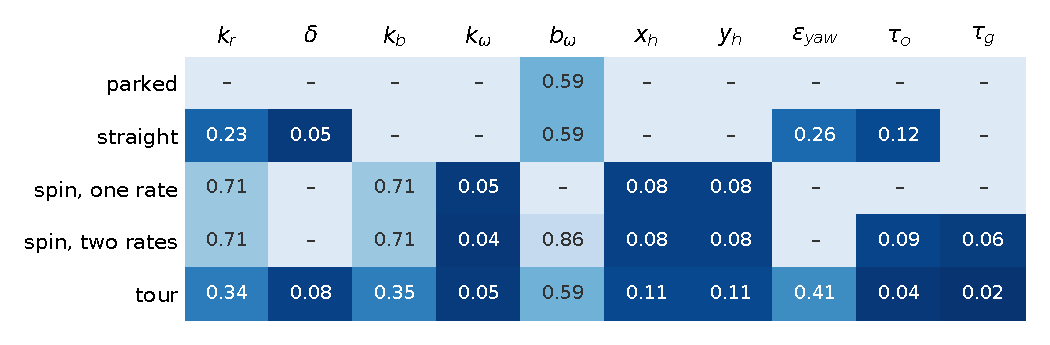
\includegraphics[width=0.86\textwidth]{d4_obs.pdf}

  \raggedright\small
  Posterior over prior sd, every other parameter estimated too; ``--'' means the motion teaches
  nothing. Standing still teaches the gyro bias and nothing else. Straight and spin teach disjoint
  sets. \alert{Observability is a property of the parameter and the motion together.}
  \src{self\_calibration.tex l.868--877, tab:sc-obs-motion; a subset of the rows}
\end{frame}

\begin{frame}{Conditional is not marginal}
  \begin{columns}[c]
    \begin{column}{0.54\textwidth}
      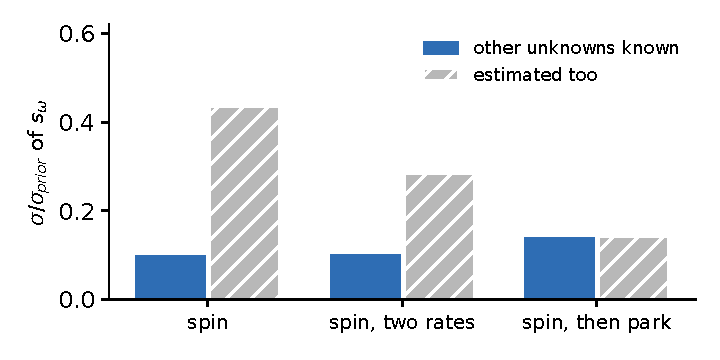
\includegraphics[width=\textwidth]{d4_schur.pdf}
    \end{column}
    \begin{column}{0.42\textwidth}
      \small
      At a constant turn rate, scale and bias both grow in proportion to time: the data see one
      combination.
      \[ S=\mathcal I_{\theta\theta}-\mathcal I_{\theta n}\,\mathcal I_{nn}^{-1}\,\mathcal I_{n\theta} \]
      The Schur complement removes what another unknown could equally have produced. A second rate,
      or a pause, splits them.
    \end{column}
  \end{columns}
  \src{self\_calibration.tex l.820--830; lab 4, exercise 18}
\end{frame}

\begin{frame}{Testing it: inject an error, and predict the recovery first}
  \[
    \text{recovery} \;=\; 1-\Big(\frac{\sigma_{\text{post}}}{\sigma_{\text{prior}}}\Big)^{\!2}
  \]
  \begin{center}
  \begin{tikzpicture}[x=6.5cm, y=0.58cm, lab/.style={font=\scriptsize}]
    \draw[muted] (0,0) -- (1.1,0);
    \foreach \v in {0,0.5,1} { \draw[muted] (\v,0) -- (\v,-0.12); \node[lab, below] at (\v,-0.12) {\v}; }
    \foreach \y/\n/\pr/\re in {3/Ricoh yaw/0.454/0.454, 2/ZED yaw/0.992/0.984} {
      \node[lab, left] at (0,\y) {\n};
      \draw[cool, very thick] (\pr,\y-0.3) -- (\pr,\y+0.3);
      \fill[accent] (\re,\y) circle (3pt);
    }
    \node[lab, left] at (0,1) {forward scale};
    \fill[accent] (1.042,1) circle (3pt);
    \node[lab, right] at (1.052,1) {104.2\% of a known 3\%};
    \draw[cool, very thick] (0.72,4.0) -- (0.72,4.5); \node[lab, right] at (0.73,4.25) {predicted};
    \fill[accent] (0.93,4.25) circle (3pt); \node[lab, right] at (0.945,4.25) {recovered};
  \end{tikzpicture}
  \end{center}
  \small
  Run twice with the same seed: the difference sees only the injection. It is predictable from the
  posterior alone, so running both checks that the estimator is consistent with itself.
  \src{self\_calibration.tex l.3056, l.3640--3644}
\end{frame}

\begin{frame}{A body that drifts, and the prior that must not move}
  \centering
  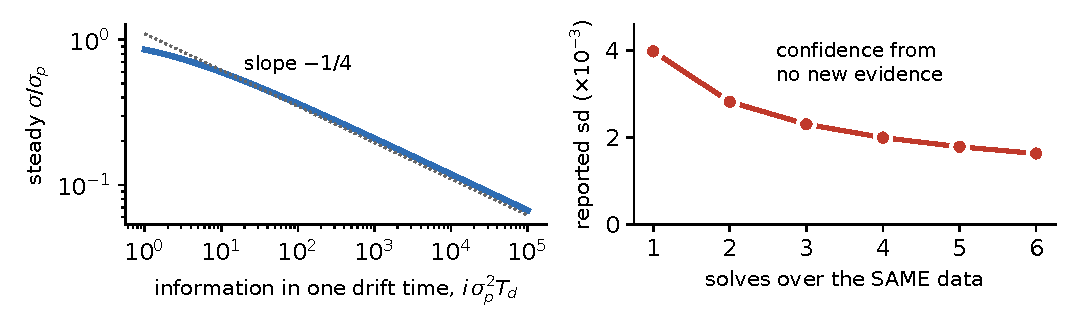
\includegraphics[width=0.88\textwidth]{d4_drift.pdf}

  \begin{columns}[T]
    \begin{column}{0.48\textwidth}
      \small
      \textbf{Drift.} A body that drifts a thousand times more slowly is tracked only about six times
      more tightly.
    \end{column}
    \begin{column}{0.48\textwidth}
      \small
      \textbf{Never re-centre a prior on its own estimate.} The same evidence counts again, and a
      parameter nothing excites wanders. \alert{Decided on the argument}: no measurement yet
      isolates the effect.
    \end{column}
  \end{columns}
  \src{self\_calibration.tex l.1001--1017, l.2763--2825; right panel: lab 4, exercise 21}
\end{frame}

\begin{frame}{Standing still is an observation}
  \begin{columns}[c]
    \begin{column}{0.5\textwidth}
      \centering\small
      \renewcommand{\arraystretch}{1.3}
      \begin{tabular}{@{}l c@{}}
        \toprule
        parameter & information per second \\
        \midrule
        $k_v$ forward scale & $v^2T/\varsigma_p^2$ \\
        $k_\omega$ heading scale & $\omega^2T/\varsigma_\theta^2$ \\
        \rowcolor{accent!15}
        $b_\omega$ gyro bias & $T/\varsigma_\theta^2$ \\
        \bottomrule
      \end{tabular}

      \vspace{0.6em}
      No rate in the last row: only time. Two legs of one route, differing in whether the robot happened
      to stand still: the data's share of the bias posterior goes from \textbf{about half} to
      \textbf{almost all}.
    \end{column}
    \begin{column}{0.46\textwidth}
      \small
      The world is sampled only where the robot looks. The body is in everything it does.

      \vspace{0.6em}
      So ordinary driving calibrates, and a manoeuvre earns its place only where the task does not
      span the covariate; a planner avoids a motion exactly as much as the motion costs it. It should
      compete with \alert{idleness}, never with a task.
    \end{column}
  \end{columns}
  \lesson{Here the one calibration action the analysis justifies is a pause.}
  \src{self\_calibration.tex l.2670--2762; active\_inference.tex l.852--868, l.957--960}
\end{frame}

% =================================================================================================
\section{Lab}
% =================================================================================================

\begin{frame}{Lab 4: paying for what you learn}
  \texttt{labs/day4.ipynb}, about two hours.
  \begin{enumerate}\small
    \item \textbf{Where to look}: $\Delta H$ on one wall, and travel priced in nats.
    \item \textbf{Priced offers}: producers publish on the graph, the controller selects; find the
          hand-offs nobody coded.
    \item \textbf{The room}: an explorer that knows when to stop, and the trap of predicting through matter.
    \item \textbf{Following}: a double pole, three ways to break it, a route deformed around an obstacle.
    \item \textbf{The body}: recover hidden wheel and gyro errors from the room's corrections; what each
          motion teaches.
  \end{enumerate}
  \vspace{0.3em}
  \small Short of time: skip exercises 2, 16, 19 and 20.
\end{frame}

\begin{frame}{Tomorrow}
  \centering
  \vspace{1em}
  {\Large The programme for Day 5 is to be confirmed.}

  \vspace{1.5em}
  \raggedright
  Today's result to carry there: \alert{what can be learnt is a property of the parameter and the
  action together}. A robot pays for what it knows; the question left is how anyone can tell whether
  it paid well.
\end{frame}

\end{document}
